

%%%%%%%%%%%%%%%%%%%%%%%%%%%%%%%%%%%%%%%%%%%%%%%%%%%%%%%%%%%%%
%%%%%%%%%%%%%%%%%%%%%%%%%%%%%%%%%%%%%%%%%%%%%%%%%%%%%%%%%%%%%
%%%%%%%%%%%%%%%%%%%%%%%%%%%%%%%%%%%%%%%%%%%%%%%%%%%%%%%%%%%%%


\begin{frame}{Local flow real-data results}

\begin{centering}
    \begin{minipage}{0.9\textwidth}
    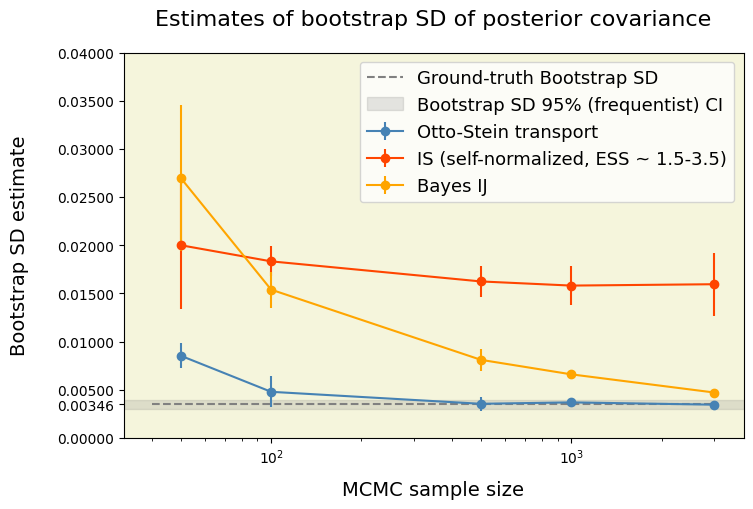
\includegraphics[width=1.0\textwidth]{static_figures/isba_poster_sens_fig.png}
    \end{minipage}
\end{centering}
\end{frame}



%%%%%%%%%%%%%%%%%%%%%%%%%%%%%%%%%%%%%%%%%%%%%%%%%%%%%%%%%%%%%
%%%%%%%%%%%%%%%%%%%%%%%%%%%%%%%%%%%%%%%%%%%%%%%%%%%%%%%%%%%%%
%%%%%%%%%%%%%%%%%%%%%%%%%%%%%%%%%%%%%%%%%%%%%%%%%%%%%%%%%%%%%





\begin{frame}{Data re-weighting.}


\onslide<1->{
Augment the problem with {\em data weights} $\w_1, \ldots, \w_N$.
We can write $\expect{\p(\theta \vert \xvec; \w)}{f(\theta)}$.
}
\onslide<1->{
%
\begin{align*}
%
\ell_n(\theta) :={}& \log \p(\x_n \vert \theta)
&
\log \p(\xvec \vert \theta; \w) ={}&
    \sumn \w_n \ell_n(\theta)
%
\end{align*}
}

\begin{minipage}{0.49\textwidth}
    \onslide<2-> {
    Original weights: \par
    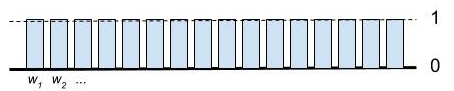
\includegraphics[width=0.78\textwidth]{static_figures/orig_weights}
    }
    \onslide<3-> {
    \par Leave-one-out weights: \par
    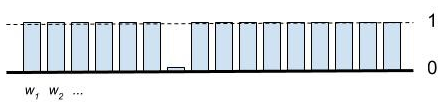
\includegraphics[width=0.78\textwidth]{static_figures/weights_loo}
    }
    \onslide<4-> {
    \par Bootstrap weights: \par
    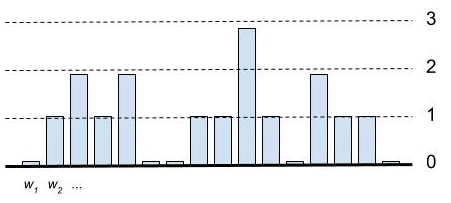
\includegraphics[width=0.78\textwidth]{static_figures/boot_weights}
    }
\end{minipage}
%\onslide<1->{
\begin{minipage}{0.49\textwidth}
    % https://www.overleaf.com/learn/latex/TikZ_package
    % https://latexdraw.com/how-to-annotate-an-image-in-latex/
    % https://tex.stackexchange.com/questions/9559/drawing-on-an-image-with-tikz
    \begin{tikzpicture}
        \onslide<5-> {
        \node[anchor=south west,inner sep=0] (image) at (0,0) {
            %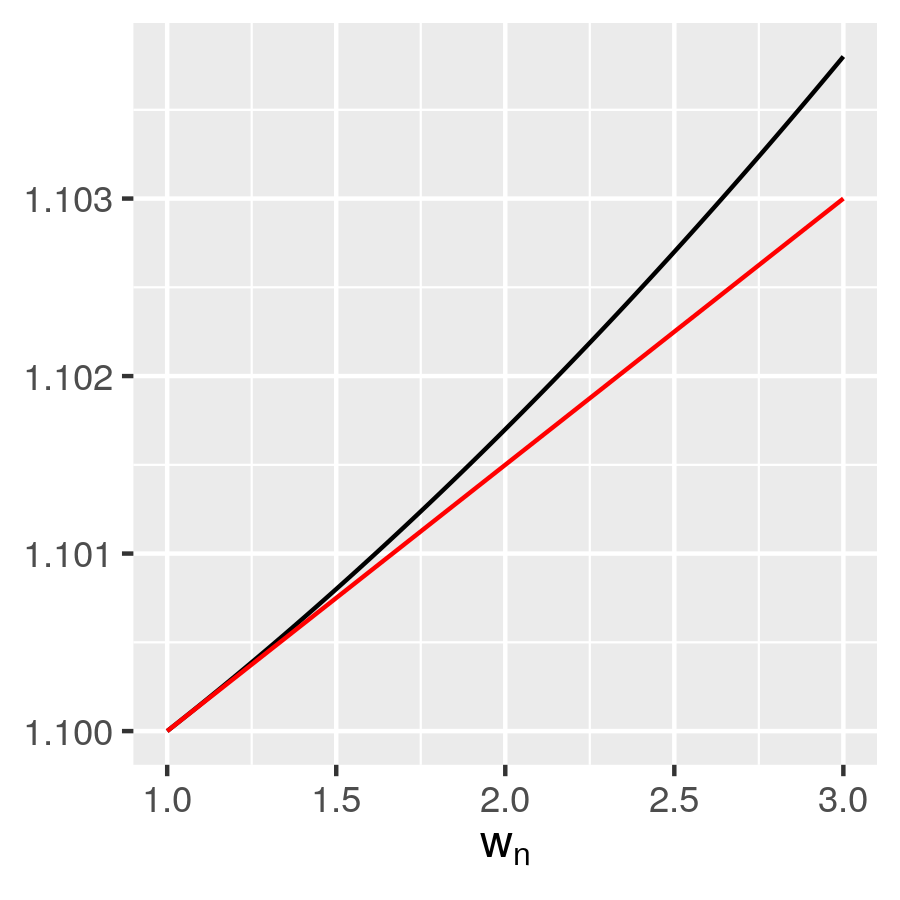
\includegraphics[width=0.98\textwidth]{static_figures/weight_slope}
            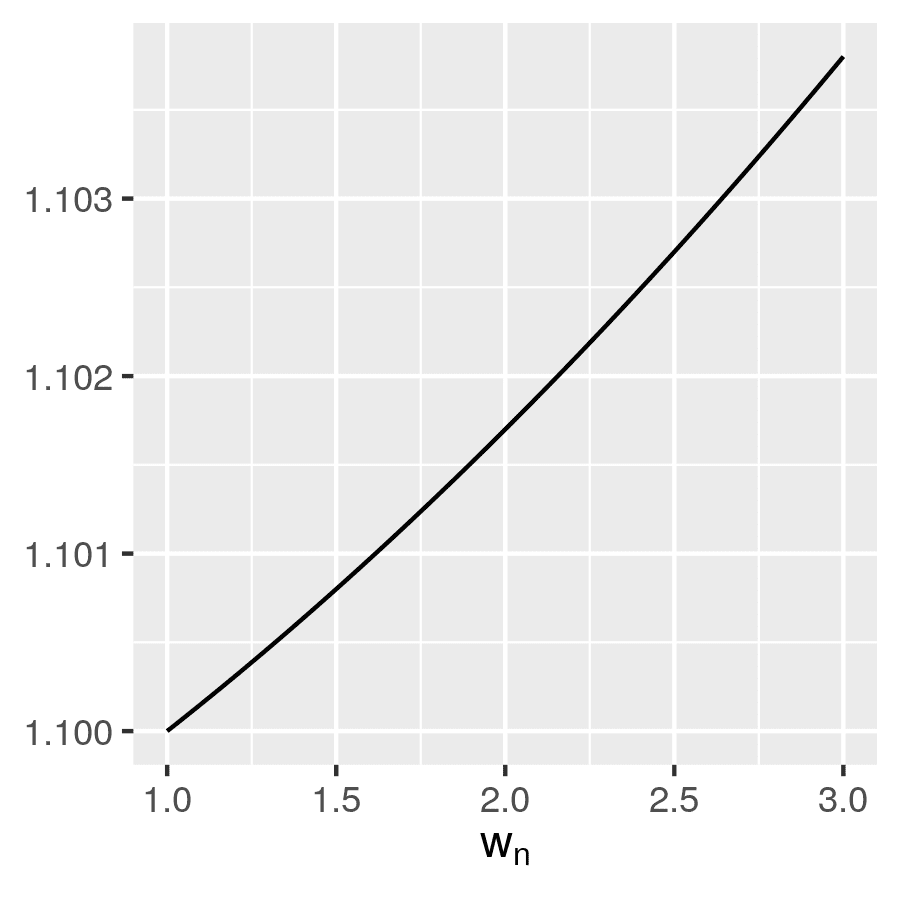
\includegraphics[width=0.98\textwidth]{static_figures/e_beta_w}
        };
        }
        \onslide<7->{
        \begin{scope}[x={(image.south east)},y={(image.north west)}]
            \draw[gray, thick, <-] (0.20,0.23) -- ++(0.15,0.3)
                    node[above,black,fill=white]
                    {\small $\expect{p(\theta \vert \xvec)}{f(\theta)}$};
        \end{scope}
        }
        \onslide<6->{
        \begin{scope}[x={(image.south east)},y={(image.north west)}]
            \draw[gray, thick, <-] (0.8,0.8) -- ++(-0.1,0.1)
                    node[left,black,fill=white]
                    {\small $\expect{p(\theta \vert \xvec; \w_n)}{f(\theta)}$};
        \end{scope}
        }
        \onslide<8->{
        \begin{scope}[x={(image.south east)},y={(image.north west)}]
            \draw[blue, thick, -] (0.18,0.18) -- ++(1.2 * 0.6, 1.2 * 0.48);
        \end{scope}
        }
        \onslide<9->{
        \begin{scope}[x={(image.south east)},y={(image.north west)}]
            \draw[gray, thick, <-] (0.4,0.35) -- ++(0.2,-0.08)
                    node[right,black,fill=white]
                    {\small Slope $ = \blue{\infl_n}$};
        \end{scope}
        }
        \onslide<10->{
        \begin{scope}[x={(image.south east)},y={(image.north west)}]
            \draw[gray, thick, <-] (0.8,0.65) -- ++(0.02,-0.2)
                    node[below,black,fill=white]
                    {\small Error $ = \red{\err_n(\w_n)}$};
            \draw[red, to-to] (0.8,0.76) -- ++(0,-0.07);
        \end{scope}
        }
    \end{tikzpicture}
%}
\end{minipage}

\onslide<11->{
The re-scaled slope $N \infl_n$ is known as the
``influence function'' at data point $\x_n$.
%
\vspace{-0.5em}
\begin{align*}
\expect{p(\theta \vert \xvec; \w)}{f(\theta)} -
    \expect{p(\theta \vert \xvec)}{f(\theta)} ={}&
    \sumn \blue{\infl_n} (\w_n - 1) +
    \red{\err_n(\w)}
    % \textrm{Higher order derivatives}
%
\end{align*}
}
%
\end{frame}


%%%%%%%%%%%%%%%%%%%%%%%%%%%%%%%%%%%%%%%%%%%%%%%%%%%%%%%%%%%%%
%%%%%%%%%%%%%%%%%%%%%%%%%%%%%%%%%%%%%%%%%%%%%%%%%%%%%%%%%%%%%
%%%%%%%%%%%%%%%%%%%%%%%%%%%%%%%%%%%%%%%%%%%%%%%%%%%%%%%%%%%%%


\begin{frame}[t]{Data re-weighting.}

\question{How can we use the approximation?}

Assume the \blue{slope} is computable and \red{error} is small.
%
%
\begin{align*}
    \expect{p(\theta \vert \xvec; \w)}{f(\theta)} -
    \expect{p(\theta \vert \xvec)}{f(\theta)} ={}&
    \sumn \blue{\infl_n} (\w_n - 1) + \red{\err_n(\w)}
\end{align*}
%
%
\pause
\textbf{Bootstrap.}
Draw bootstrap
weights $\w \sim \p(\w) = \textrm{Multinomial}(N, N^{-1})$.
%
\begin{align*}
%
\textrm{Bootstrap variance} ={}&
\var{\p(\w)}{\expect{p(\theta \vert \xvec; \w)}{f(\theta)}}
\onslide<3->{
\\={}&
\var{\p(\w)}{
    \sumn \blue{\infl_n} (\w_n - 1) + \red{\err_n(\w)}
}
\\=& 
\frac{1}{N^2} \sumn \left(
    \blue{\infl_n - \overline{\infl}}
\right)^2 +
\red{\textrm{Term involving }
    \red{\err_n}(\w)
    \textrm{ for }n =1,\dots,N
}
\\\red{\approx}{}&
\frac{1}{N}
\undernote{
    \left( 
    \frac{1}{N} \sumn \left(
        \blue{\infl_n - \overline{\infl}}
    \right)^2
    \right)
}{\textrm{``Infinitesimal jackknife variance estimate''}}
}
%
\end{align*}
    
\end{frame}

    




% %%%%%%%%%%%%%%%%%%%%%%%%%%%%%%%%%%%%%%%%%%%%%%%%%%%%%%%%%%%%%%%%%%%%%%%%%%%
% %%%%%%%%%%%%%%%%%%%%%%%%%%%%%%%%%%%%%%%%%%%%%%%%%%%%%%%%%%%%%%%%%%%%%%%%%%%
% %%%%%%%%%%%%%%%%%%%%%%%%%%%%%%%%%%%%%%%%%%%%%%%%%%%%%%%%%%%%%%%%%%%%%%%%%%%

\begin{frame}[t]{Bayesian posterior functionals}

Supppose we are interested in $\expect{\post}{\g(\theta)}$.
Let the regression log likelihood be $\ell(\y \vert \x, \theta)$.\\[1em]

\generalizedpost{}

Let $\psurhat$ denote the empirical distribution over $\x_i, \y_i$.  Then
%
\begin{align*}
    \T(\psurhat, \nsur) =
    \frac{
        \int \g(\theta) \exp\left( \nsur \meansur \ell(\y_i \vert \x_i, \theta) \right)
            \prior(\theta) d\theta
    }
    {
    \int \exp\left( \nsur \meansur \ell(\y_i \vert \x_i, \theta) \right)
        \prior(\theta) d\theta
    } = \expect{\post}{\g(\theta)}.
\end{align*}


Consider a smooth path of densities $\epsilon \mapsto \p^\epsilon$. 
The directional derivative in general is
$$
\begin{aligned}
\fracat{\partial \T(\p^\epsilon, N)}{\partial \epsilon}{\epsilon=0} ={}&
    \cov{\p(\theta \vert \p, N)}{
        \g(\theta), 
        N \int \ell(\yn \vert \xn, \theta) \w(d \xn)
        \fracat{\partial \log \p_\epsilon(\yn \vert \xn)}
               {\partial \epsilon}{\epsilon = 0} d\xn d\yn
    }
\\\Rightarrow
\fracat{\partial \T({\psurhat}^\epsilon, \nsur)}{\partial \epsilon}{\epsilon=0} ={}&
    \cov{\post}{
        \g(\theta), 
        \sumsur \ell(\y_i \vert \x_i, \theta)
        \fracat{\partial \log {\psurhat}^\epsilon(\y_i \vert \x_i)}
               {\partial \epsilon}{\epsilon = 0}
    }
\end{aligned}
$$

\end{frame}



% %%%%%%%%%%%%%%%%%%%%%%%%%%%%%%%%%%%%%%%%%%%%%%%%%%%%%%%%%%%%%%%%%%%%%%%%%%%
% %%%%%%%%%%%%%%%%%%%%%%%%%%%%%%%%%%%%%%%%%%%%%%%%%%%%%%%%%%%%%%%%%%%%%%%%%%%
% %%%%%%%%%%%%%%%%%%%%%%%%%%%%%%%%%%%%%%%%%%%%%%%%%%%%%%%%%%%%%%%%%%%%%%%%%%%

\begin{frame}[t]{Bayesian posterior functionals}

We're interested in $\g(\theta) = \meantar \m(\theta^\trans \x_j)$.

For some function $\w(\xn)$, set
$$
\psur^\epsilon(\xn, \yn) = 
    \psur(\xn, \yn) + \epsilon \w(d \xn) \psur(\xn, \yn) =
    \left( \psur(\xn) + \epsilon \w(\xn) \right) \psur(\yn \vert \xn).
$$
This is a shift in the marginal distribution of $\x$ in the direction $\w(\x)$,
with\\[1em]
$$
\begin{aligned}
    \fracat{\partial \psur^\epsilon(\yn \vert \xn)}
               {\partial \epsilon}{\epsilon = 0} =
               \w(\xn) \psur(\yn \vert \xn).
\end{aligned}
$$

Our diagnostic is then given by
$$
\Delta(\p) =
    \cov{\p(\theta)}{
        \meantar \m(\theta^\trans \x_j),
        N \int \ell(\yn \vert \xn, \theta) \psur(\yn \vert \xn) \w(\xn) d \xn \, d \yn
        }
$$
%
\end{frame}




%%%%%%%%%%%%%%%%%%%%%%%%%%%%%%%%%%%%%%%%%%%%%%%%%%%%%%%%%%%%%%%%%%%%%%%%%%%
%%%%%%%%%%%%%%%%%%%%%%%%%%%%%%%%%%%%%%%%%%%%%%%%%%%%%%%%%%%%%%%%%%%%%%%%%%%
%%%%%%%%%%%%%%%%%%%%%%%%%%%%%%%%%%%%%%%%%%%%%%%%%%%%%%%%%%%%%%%%%%%%%%%%%%%

\begin{frame}{Exchangeable units: Experimental results revisited}
    Our results were actually computed on \textbf{identical datasets}
    with $G = N$ and $g_n=n$.

    \begin{center}
    \begin{minipage}{0.34\textwidth}
        Uses $\log \p(\x_n \vert \gamma)$:\\
        $\infl_n = \expect{\p(\gamma \vert \xvec)}{\gammabar \ellbar_n(\gamma)}$

        \onslide<2->{
        \spskip
        Not easily computable from\\
        $\gamma, \lambda \sim \p(\gamma, \lambda \vert \xvec)$\\
        in general.
        }
    \end{minipage}
    \begin{minipage}{0.65\textwidth}
        \LowDimAccuracyGraph{}
        % \HighDimAccuracyGraph{}
    \end{minipage}
    %

    \begin{minipage}{0.34\textwidth}
        Uses $\log \p(\x_n \vert \gamma, \lambda)$:\\
        $\infl_n = \expect{\p(\gamma,\lambda \vert \xvec)}{\gammabar \ellbar_n(\gamma, \lambda)}$

        \onslide<2->{
        \spskip
        Easily computable from\\
        $\gamma, \lambda \sim \p(\gamma, \lambda \vert \xvec)$.
        }

        \onslide<3->{
        \spskip
        May still be useful when $\p(\lambda \vert \xvec)$
        is {\em somewhat} concentrated.
        }

    \end{minipage}
    \begin{minipage}{0.65\textwidth}
        %\LowDimAccuracyGraph{}
        \HighDimAccuracyGraph{}
    \end{minipage}
    %
\end{center}
    %
\end{frame}




\begin{frame}{High dimensional problems}
    %
    \question{Example: Exponential families  with random effects (REs)
    $\lambda$ and fixed effects $\gamma$.}

    If the observations per random effect remains bounded as $N \rightarrow
    \infty$, then
    %
    \begin{itemize}
    %
    \item Parameter $\lambda$ (``local'') grows in dimension with $N$.
    \item Parameter $\gamma$ (``global'') is finite-dimensional.
    \item Marginally $\p(\lambda \vert \xvec)$ does not concentrate.
    \item Marginally, $\p(\gamma \vert \xvec)$ concentrates.
    % \item Conditionally, $\p(\lambda \vert \gamma, \xvec)$ does not concentrate either.
    %
    \end{itemize}
    

\spskip
\pause
\question{
In general, we cannot hope for an asymptotic analysis of
    $\expect{\p(\lambda, \gamma \vert \xvec)}{f(\lambda)}$. \\
%
\spskip
Can we save the approximation when {\em some} parameters concentrate?\\
%
\spskip
Does the residual vanish asymptotically for
$\w_n \mapsto \expect{\p(\gamma \vert \xvec; \w_n)}{f(\gamma)}$?
}

%
\end{frame}




%%%%%%%%%%%%%%%%%%%%%%%%%%%%%%%%%%%%%%%%%%%%%%%%%%%%%%%%%%%%%%%%%%%%%%%%%%%%%%
%%%%%%%%%%%%%%%%%%%%%%%%%%%%%%%%%%%%%%%%%%%%%%%%%%%%%%%%%%%%%%%%%%%%%%%%%%%%%%
%%%%%%%%%%%%%%%%%%%%%%%%%%%%%%%%%%%%%%%%%%%%%%%%%%%%%%%%%%%%%%%%%%%%%%%%%%%%%%

\begin{frame}{High dimensional problems}
%
We assume that $\p(\gamma \vert \xvec)$ concentrates but
$\p(\lambda \vert \xvec)$ does not.  By our series expansion:
%
\begin{align*}
%
% \MoveEqLeft
&
\expect{\p(\gamma, \lambda \vert \xvec; \w_n)}{\gamma} -
\expect{\p(\gamma, \lambda \vert \xvec)}{\gamma}
={}
\\
&\quad\blue{\infl_n}(\w_n - 1) && +\red{\err_n(\w)}
% \\&
\onslide<2->{
\\={}&
\blue{
\expect{\p(\gamma, \lambda \vert \xvec)}{
    \gammabar \ellbar_n(\gamma,\lambda)}
}
(\w_n - 1)
    && +
    \frac{1}{2}
    \red{
    \expect{\p(\gamma, \lambda \vert \xvec; \wtil_n)}{
        \gammabar
        \ellbar_n(\gamma,\lambda)^2 }
    }
        (\w_n - 1)^2
% \\&
}
\onslide<3->{
\\={}&
%
\blue{
\expectop{\p(\gamma \vert \xvec)} \Big[
    \gammabar
    \undernote{
        \expect{\p(\lambda \vert \gamma, \xvec)}
                {\ellbar_n(\gamma,\lambda)}
            }{F_1(\gamma)}
    \Big]
}
        (\w_n - 1)
    && +
    \frac{1}{2}
    \red{
    \expectop{\p(\gamma \vert \xvec; \wtil_n)} \Big[
        \gammabar
        \undernote{
            \expect{\p(\lambda \vert \xvec, \gamma; \wtil_n)}{
                \ellbar_n(\gamma,\lambda)^2}
            }{F_2(\gamma)}
        \Big]
    }
        (\w_n - 1)^2
}
\onslide<4->{
\\={}&
\undernote{
\blue{
\expect{\p(\gamma \vert \xvec)}{
    \gammabar F_1(\gamma)}
}
}{O_p(N^{-1})\\\text{(by $\p(\gamma \vert \xvec)$ concentration)}}
    (\w_n - 1)
    && +
    \frac{1}{2}
\undernote{
\red{
\expect{\p(\gamma \vert \xvec; \wtil_n)}{
    \gammabar
    F_2(\gamma) }
}
}{O_p(N^{-1})\\\text{(by $\p(\gamma \vert \xvec)$ concentration)}}
        (\w_n - 1)^2
%
\\& \Rightarrow
}
\onslide<5->{
\blue{\infl_n = O_p(N^{-1})} &&
\red{\err_n(\w) = O_p(N^{-1})}
}
%
\end{align*}
%
\onslide<6->{
% The error is the same order as the linear approximation, and does not vanish after rescaling!

\theorem{
    \textbf{Corollary \parencite{giordano:2023:bayesij}:}\\
    In general, $\w_n \mapsto N \left( \expect{\p(\gamma \vert \xvec; \w_n)}{\gamma} -
    \expect{\p(\gamma \vert \xvec)}{\gamma} \right)$
    remains non-linear as $N \rightarrow \infty$.    
}

}

\end{frame}



%%%%%%%%%%%%%%%%%%%%%%%%%%%%%%%%%%%%%%%%%%%%%%%%%%%%%%%%%%%%%%%%%%%%%%%%%%%
%%%%%%%%%%%%%%%%%%%%%%%%%%%%%%%%%%%%%%%%%%%%%%%%%%%%%%%%%%%%%%%%%%%%%%%%%%%
%%%%%%%%%%%%%%%%%%%%%%%%%%%%%%%%%%%%%%%%%%%%%%%%%%%%%%%%%%%%%%%%%%%%%%%%%%%

\begin{frame}{Example: Poisson regression with Gamma-distributed random effects}
    %
    \begin{align*}
    \textrm{For }g=1,\ldots,G,\textrm{ }
        \lambda_g \iid{}& \mathrm{Gamma}(\alpha, \beta) \textrm{ for fixed }\alpha,\beta\\
    \textrm{For }n = 1,\ldots,N,\textrm{ }
        g_n \iid{}& \mathrm{Categorical}(1,\ldots,G),\textrm{ }
        y_n | \lambda_n, \gamma, g_n \iid{}
            \mathrm{Poisson}(\gamma \lambda_{g_n}).\\
    \x_n ={} (y_n, g_n)
    \textrm{ are IID given } \lambda, \gamma. &
    \textrm{   Write }\log \p(\xvec \vert \lambda, \gamma; \w) =
       \sumn \w_n \ell_n(\lambda, \gamma).
    %
    \end{align*}
    
    \pause
    
    \HighDimAccuracyGraph{}
    
\end{frame}
        



% von Mises stuff
\def\gdist{\mathbb{G}}
\def\fndist{\mathbb{F}_N}
\def\ftdist{\mathbb{F}_N^{\t}}
\def\fwdist{\mathbb{F}_{N}^{w}}
\def\T{T}   % Stastistical functional
\def\Tlin{T_{\mathrm{lin}}} % linearized functional
\def\t{t}   % Path variable for von Mises expansion
\def\g{g}   % Function of interest
\def\xn{\x_{0}}   % Function of interest
\def\prior{\pi}
\def\ttil{\tilde{\t}}   % IVT value of t
% \def\abs#1{\left\vert #1\right\vert }


%%%%%%%%%%%%%%%%%%%%%%%%%%%%%%%%%%%%%%%%%%%%%%%%%%%%%%%%%%%%%%%%%%%%%%%%%%%
%%%%%%%%%%%%%%%%%%%%%%%%%%%%%%%%%%%%%%%%%%%%%%%%%%%%%%%%%%%%%%%%%%%%%%%%%%%
%%%%%%%%%%%%%%%%%%%%%%%%%%%%%%%%%%%%%%%%%%%%%%%%%%%%%%%%%%%%%%%%%%%%%%%%%%%



%%%%%%%%%%%%%%%%%%%%%%%%%%%%%%%%%%%%%%%%%%%%%%%%%%%%%%%%%%%%%%%%%%%%%%%%%%%
%%%%%%%%%%%%%%%%%%%%%%%%%%%%%%%%%%%%%%%%%%%%%%%%%%%%%%%%%%%%%%%%%%%%%%%%%%%
%%%%%%%%%%%%%%%%%%%%%%%%%%%%%%%%%%%%%%%%%%%%%%%%%%%%%%%%%%%%%%%%%%%%%%%%%%%




\begin{frame}[t]{Bayesian von--Mises Expansion Results}

\theorem{
    \textbf{Theorem 3 \parencite{giordano:2023:bayesij} (sketch): }\\
    \textbf{(Consistency of the von--Mises expansion in finite dimensions) }\\
    Under slightly stronger conditions our original finite--dimensional posterior 
    consistency result, 
    %
\begin{align*}
    \sup_{\ttil \in [0,1]} | \red{\err(\ttil)} | \rightarrow 0
    \quad\textrm{in the Bayesian von--Mises expansion.}
\end{align*}
%
}

\pause

\theorem{
\textbf{Theorem 4 \parencite{giordano:2023:bayesij} (sketch):}\\
\textbf{(Inconsistency of the von--Mises expansion in high dimensional exponential families) }\\
    Assume that $\x_n$ comes with a equiprobable group assignment $g_n \in 1,\ldots,G$.\\    
    Conditional on $g$, $\x_n$ is modeled as a finite-dimensional exponential
    family given $\lambda,\gamma$:
    %
    \begin{align*}
        \log \p(x_n \vert g_n=g, \gamma, \lambda) = 
            \tau(x_n)^\trans \eta_{g}(\gamma, \lambda) + \textrm{Constant}.
    \end{align*}
    %
Define the average product of second moments:
%
\begin{align*}
    \mathcal{V}_N(\gamma) :=
    \frac{1}{G} \sum_{g=1}^G 
    \trace{
        \expect{\fdist(\x_n)}{\tau(\x_n) \tau(\x_n)^\trans}
        \cov{\p(\lambda \vert \gamma, \fdist)}{\eta_{g}(\gamma, \lambda)}
    }.
\end{align*}
%
If $N \expect{\p(\gamma \vert \fdist)}{\fbar(\gamma) \mathcal{V}_N(\gamma)}$ is 
strictly bounded away from $0$ as $N\rightarrow \infty$, then
%
\begin{align*}
    \sup_{\ttil \in [0,1]} | \red{\err(\ttil)} | \rightarrow \infty
    \quad\textrm{in the Bayesian von--Mises expansion.}
\end{align*}
%
}

\end{frame}



    
%%%%%%%%%%%%%%%%%%%%%%%%%%%%%%%%%%%%%%%%%%%%%%%%%%%%%%%%%%%%%%%%%%%%%%%%%%%
%%%%%%%%%%%%%%%%%%%%%%%%%%%%%%%%%%%%%%%%%%%%%%%%%%%%%%%%%%%%%%%%%%%%%%%%%%%
%%%%%%%%%%%%%%%%%%%%%%%%%%%%%%%%%%%%%%%%%%%%%%%%%%%%%%%%%%%%%%%%%%%%%%%%%%%


% \begin{frame}{More experimental results for Gamma--Poisson mixtures}
%     \begin{minipage}[c]{0.35\textwidth}
%         We ran simulations of the Gamma--Poisson mixture with
%         different ratios of $N / G$ \\(average observations per group).

%         \spskip
%         %
%         \begin{itemize}
%             \item When $N/G$ is small:
%             %
%             \begin{itemize}
%                 \item IJ is biased significantly downwards
%                 \item Bootstrap is biased somewhat downwards
%             \end{itemize}
%             %
%             \item When $N/G$ is larger:
%             %
%             \begin{itemize}
%                 \item Both improve
%                 \item Both remain somewhat biased
%                 \item The IJ and bootstrap perform similarly
%             \end{itemize}
%             %
%         \end{itemize}
%     %
%     \end{minipage}
%     \begin{minipage}[c]{0.6\textwidth}
%     \PoissonREGraph{}
%     \end{minipage}
% \end{frame}



